\section{Summary}

This work is ongoing and is in preparation for publication.

The goal of this work is to investigate and measure the size-diffusivity relationship of single-molcules in a confined environment. The goal of this project was to better understand the biases, variance, and details of size measurements performed by convex-lens induced confinement (CLiC). 

This study overviews a the dynamics on a model particle, which was chosen as plastic beads. The ionic concentration, as discussed in Chp. [5], is very important in focusing particles into an effective confinement length. This paper tends to evalute this model experimentally, as the Langevin model, although complete, is not-trivial in fuzzy/applied systems. To show this, the method is applied to 3 species of lipid-nanoparticle sample - liposomal, spherical, and bleb-like topologies.

During experimental trails, it has been found that these samples tend to stick to negatively charged surfaces, such as negatively charged cover glass, due to Van der Walls forces and electrostatic interactions. Over the last decade, passivation methods were used to alleviate this sticking. This paper aims to measure these interactions to determine the biases on size characterization associated with measuring molecule size in systems with these passivation methods. 


\section{Methods}

The following section outlines the tools used to collect data for this thesis. 

\subsection{Aparatus schematic}

The schematic of the system is Here we re-draw Fig \ref{fig:schematic} to remind the reader of the system. The optical system used for imaging is an iSCAT microscope. 

The optical system consisted of a $\SI{405}{\nm}$ excitation laser. The output of the laser was $\SI{240}{\milli \watt}$ pre-spatial filter, with an output of $\SI{120}{\milli \watt}$ post-spatial filter. The objective used was the $100 \times$ oil imaging objective (Nikon, Apochromat TIRF $100 \times$ oil immersion objective N.A. 1.49, W.D. $\SI{0.12}{\mm}$, F.O.V $\SI{22}{\mm}$). The camera used was the (\textcolor{red}{PRODUCT ID}) CMOS camera. Operating software was custom written by (\textcolor{red}{Author}) in LabView. 

\begin{figure}[t]
	\centering
    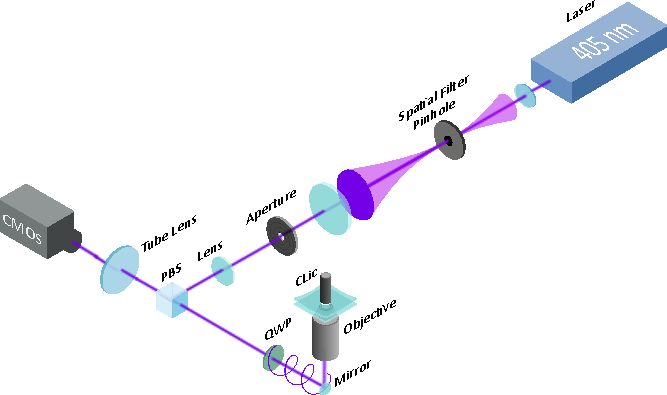
\includegraphics[width=\linewidth]{Figures/schematic}
    \caption{ iSCAT Schematic. A 405 nm laser is sent through a spatial filter, passes through an aperture. The beam is sent through a focusing lens which is reflected off a polarizing beam splitter, polarized through a QWP focused on the back plane of the objective. The scattered light is then polarized again, passing through the polarizing beam splitter and is focused on the CMOS camera. The final image is collected via the CMOS and saved in binary format.}
	\label{fig:re_schematic}
\end{figure}


\subsection{Cover-Glass}

The flow-cell device consisted of two glass substrates (Ted Pella, product no.260372, $145 \pm \SI{15}{\micro \meter}$ thick, $25 \times \SI{25}{\mm}$ cover glass), separated by a 30 um thick double-sided adhesive spacer (Nitto Denko, product no. 5603). 

\subsection{Convex-lens induced confinement}

The CLiC system was used to achieve nanometer confinement while imaging. This method is described in detail in the seminal publication \cite{berardPrecisionPlatformConvex2013}. A convex pusher lens is used together with a piezo linear actuator to displace the top coverslip of the flow-cell in a parabolic displacement. The pieze actuator is manually controlled during imaging and set to a specific, controlled height. The height is determined using the inference fringes of Newton's rings. The full method outline is visualized in Fig. \ref{fig:c7_fig1}


\begin{figure}
    \centering
    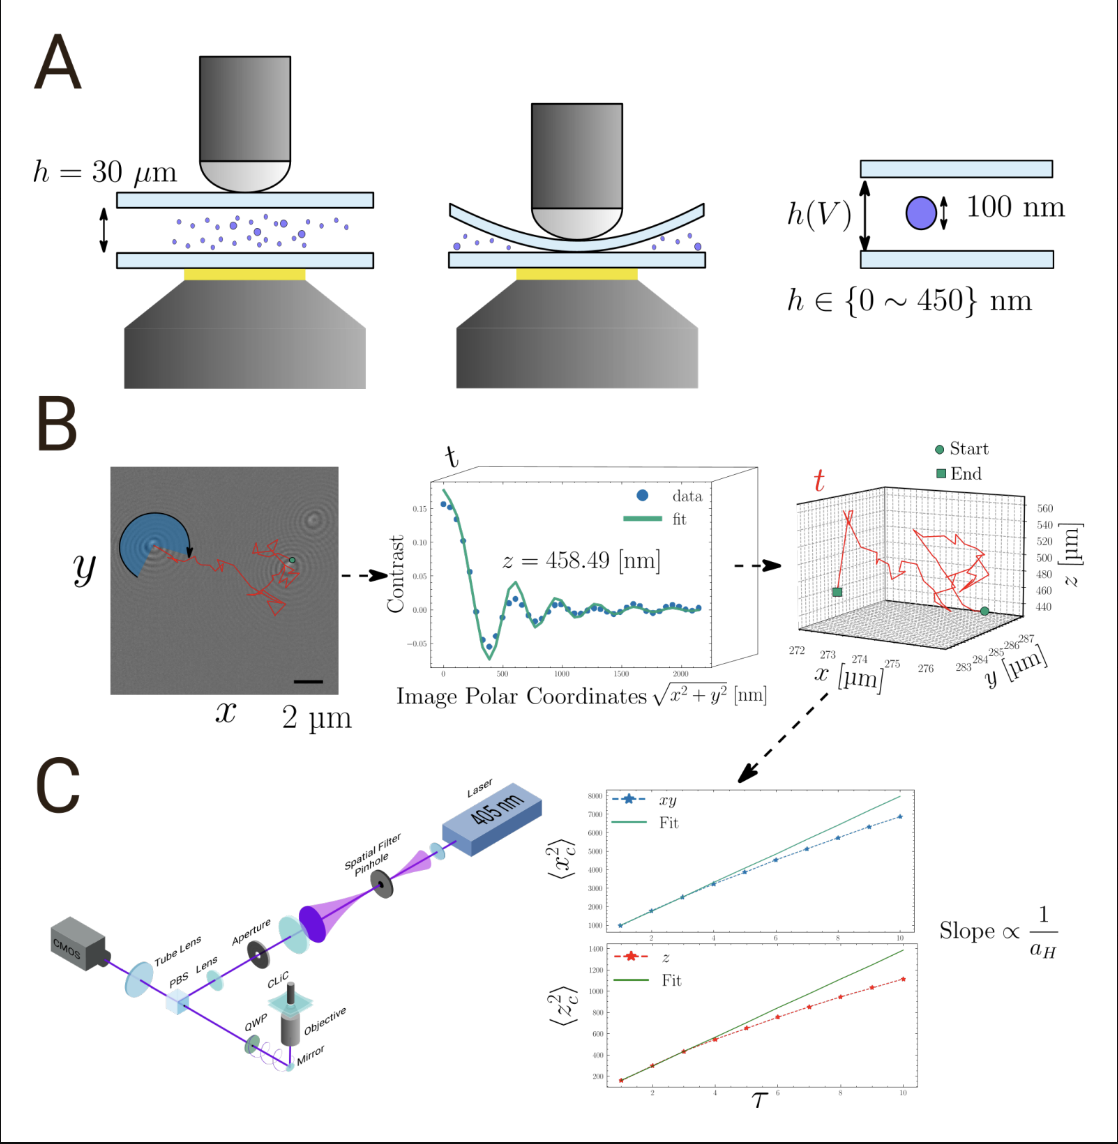
\includegraphics[width=\textwidth]{Figures/c7_overview.png}
    \caption{Figure Caption.}
    \label{fig:c7_fig1}
\end{figure}

\subsection{Sample Details}
The samples used in this thesis are listed below. Carboxylate modified polystyrene beads were purchased from thermofisher (FluoSpheres\texttrademark carboxylate-modified microspheres, Catalog No. F8799, are $\SI{0.1}{\micro \meter}$ polystyrene beads). Sample consists of $\SI{0.1}{\micro \meter}$ polystyrene beads with $\SI{500}{\micro \meter}$ dfluorescent tag attached. The tag is attached as that is what the lab had and has used in prior measurements. The beads were able to be measured in de-ionized water (MilliQ), as well as a concentration series of phosphate-buffered saline. 

Lipid-nanopartilces used in this thesis were formulated by the Pieter Cullis lab. The liposomal formulation was used as liposomal (20\% norMC3). The spherical, oil-core LNP, is the Onpattro (50\% norMC3) LNP formulation made with 25 mM NaOAc. The bleb-like LNP is the Onpattro bleb (50\% norMC3) LNP formulation made with 300 mM NaOAc. (Cryo (?)).

\section{Results}

im not sure at the moment. 

\section{Discussion of Results}